\chapter{Related Work}
\label{chap:related-work}

Based on the background provided in Section \ref{sect:comp-vision-tasks}, the extraction of semantic fractures in end-to-end detectors, such as the \textbf{one-stage detector} and \textbf{two-stage detector}, is accomplished using a \textit{backbone}. This is followed by an attached \textit{neck} that fuses features from various layers of the backbone, as depicted in Figure \ref{fig:net-backbone-neck-head}.
In this chapter, we will delve into the combined use of the backbone and neck in one of the state-of-the-art \textbf{two-stage detector}, \textit{Mask R-CNN}~\cite{DBLP:journals/corr/HeGDG17}.

\begin{figure}[htb]
    \centering
    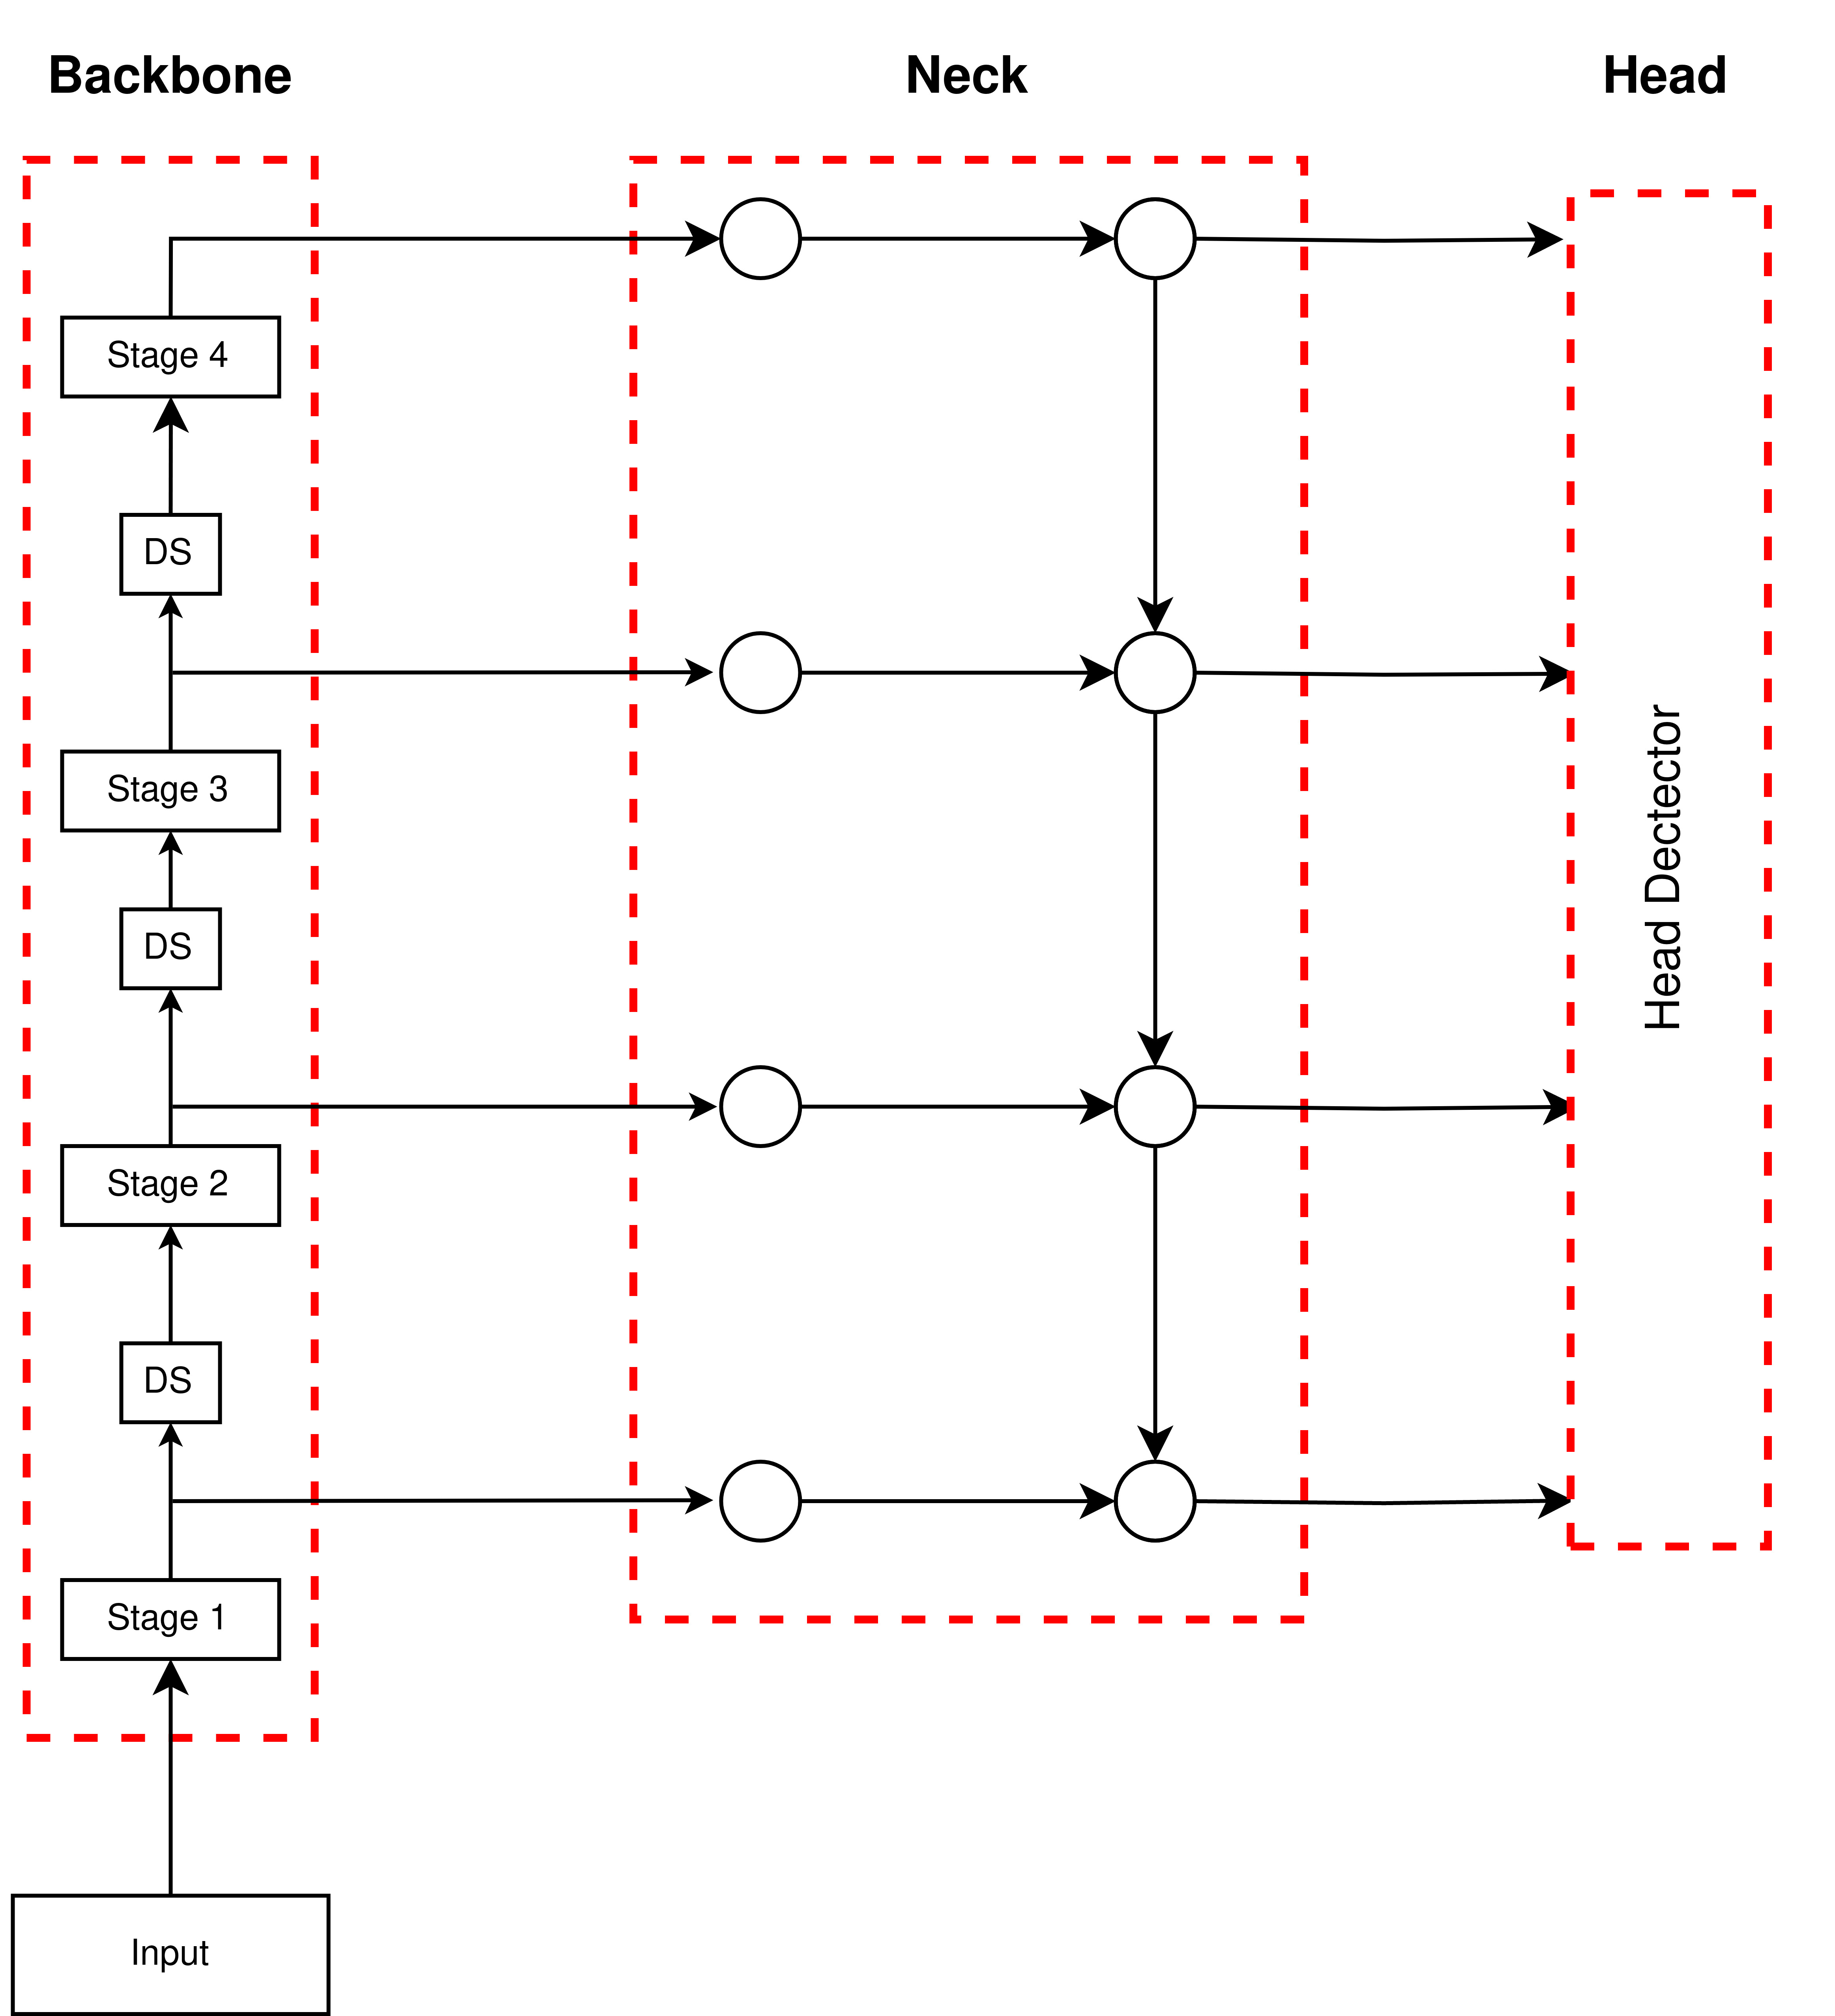
\includegraphics[width=0.6\linewidth]{figures/chapters-imgs/30/net-backbone-neck-head.jpg}
    \caption{Diagram illustrating the architecture of an end-to-end detector, featuring a \textit{backbone}, a \textit{neck}, and a \textit{head} for detection functions.}
    \label{fig:net-backbone-neck-head}
\end{figure}

\section{Backbones}
Feature extraction from images serves as the foundational step in deep learning networks tailored for computer vision tasks, as elaborated in the previous chapter. This ability of the network to extract features can be generalized to various tasks through transfer learning~\cite{DBLP:journals/corr/YosinskiCBL14}. This creates a robust network that can be adapted for multiple tasks without the need for retraining every time. Given this, a \textbf{backbone} can be defined as a pre-trained network dedicated to feature extraction and has been fine-tuned across multiple tasks prior to its designated use.

For the scope of this work, we will employ three cutting-edge backbones: InternImage~\cite{wang2023internimage}, ConvNeXt~\cite{liu2022convnet}, and EfficientNetV2~\cite{tan2021efficientnetv2}.

\subsection{InternImage}
\textit{Wenhai Wang et al.} introduced their model, \textit{InternImage}~\cite{wang2023internimage}, designed to efficiently scale with larger parameter sizes and learn potent representations from vast training data. This approach achieved representations that are comparable to, if not better than, large-scale \textit{ViTs}~\cite{dosovitskiy2021image, liu2021swin, Wang_2022, zhai2022scaling}.

In transformer-based architectures, the global attention mechanism employed by \textit{ViT}~\cite{dosovitskiy2021image} often incurs high computational and memory overheads, particularly with extensive feature maps. This burden restricts its utility in many downstream applications.

Addressing this issue, \textit{InternImage} aims to resolve the challenges of long-range dependencies and adaptive spatial aggregation inherent to the multi-head self attention (MHSA)~\cite{vaswani2023attention} operator frequently found in transformer-based architectures. Their solution harnesses an advanced version of the Deformable Convolution v2 (DCNv2)~\cite{zhu2018deformable} operator named DCNv3. This enhanced operator compensates for the limitations of standard convolution in handling long-range dependencies and adaptive spatial aggregation. Furthermore, it retains the inductive bias of traditional convolution and employs sparse sampling, proving to be more computationally memory-efficient compared to operators like \textit{MHSA}.\\

\begin{figure}[htb]
    \centering
    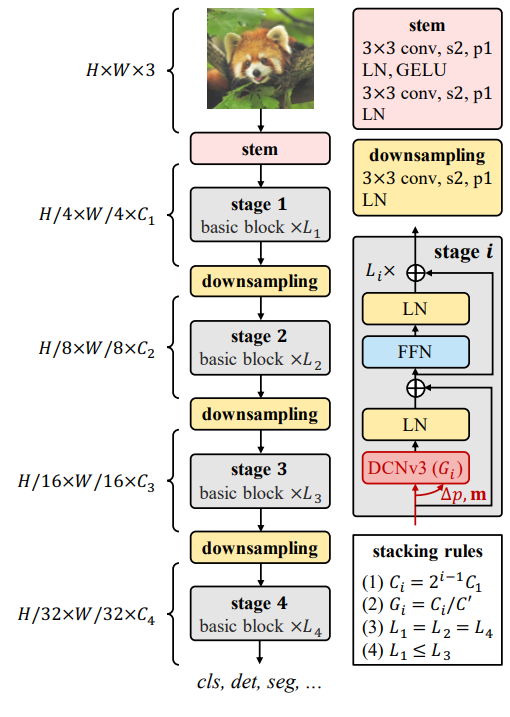
\includegraphics[width=0.6\linewidth]{figures/chapters-imgs/30/internimage-arq.png}
    \caption[\textit{InternImage} architecture]{A schematic representation of the \textit{InternImage} architecture detailing its four distinct stages. Image adapted from~\cite{wang2023internimage}.}
    \label{fig:internimage-arq}
\end{figure}

The \textit{InternImage} architecture comprises a series of stacked basic blocks, complemented by a stem and down-sampling layers, as illustrated in Figure \ref{fig:internimage-arq}. These basic blocks incorporate Layer Normalization~\cite{ba2016layer}, a feed-forward network (akin to the one used in transformer-based architectures~\cite{vaswani2023attention}), and are activated using GELU~\cite{hendrycks2023gaussian}. To generate hierarchical feature maps, the architecture employs a convolutional stem and down-sampling layers, which resize the feature maps across various scales.\\

For the purposes of this study, we will employ the \textit{InternImage-S} backbone, which consists of approximately $50M$ parameters. This model has been trained on the classification task using the \textit{ImageNet-1K} dataset~\cite{5206848} for 300 epochs.

\subsection{ConvNeXt} \label{sec:rw:convnext}
\textit{Zhuang Liu et al.} undertook a thorough reassessment of the Convolutional Neural Network's design landscape in their pioneer work, introducing the ConvNeXt architecture~\cite{liu2022convnet}. Within this exploration, the authors meticulously examined the architectural differences that distinguish convolutional models from transformer-based counterparts. Stemming from their investigation, they presented the ConvNeXt, a novel \textit{family of pure ConvNets}.\\

The ConvNeXt architectures share similarities at the micro level with transformer-based models such as \textit{DeiT}~\cite{touvron2021training} and \textit{Swin}~\cite{liu2021swin}. Common features include the GELU activation~\cite{hendrycks2023gaussian}, the integration of Layer Normalization~\cite{ba2016layer}, and distinct down-sampling layers dedicated to feature resolution adjustments. On the other hand, when observed from a macro perspective, the ConvNeXt architectures draw parallels with the \textit{ResNeXt}~\cite{8100117} structure. They predominantly employ techniques like grouped convolution and depth-wise convolution as the central operations within their stage blocks, a design which is visually detailed in Figure \ref{fig:convnext-block}.\\

\begin{figure}[htb]
    \centering
    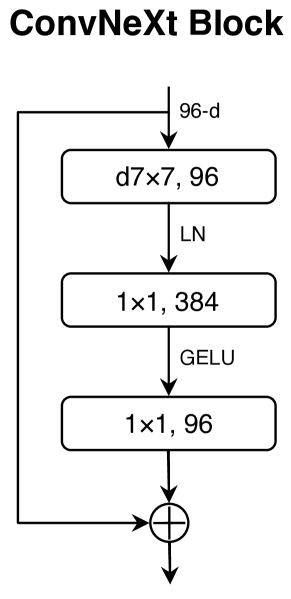
\includegraphics[width=0.25\linewidth]{figures/chapters-imgs/30/convnext-block.png}
    \caption{Block design for a \textit{ConvNeXt}. Image adapted from~\cite{wang2023internimage}.}
    \label{fig:convnext-block}
\end{figure}

In the context of our current research, we have opted to utilize the \textit{ConvNeXt-S} backbone, a robust model encompassing roughly $50M$ parameters. Prior to its deployment, the model underwent an intensive pre-training phase focused on the classification task, leveraging the expansive \textit{ImageNet-21K} dataset~\cite{5206848}. This pre-training lasted for 90 epochs. Subsequently, to further refine its capabilities, it was trained on the \textit{ImageNet-1K} dataset for 300 epochs.

\subsection{EfficientNetV2}
In the domain of deep learning models, retraining often poses significant challenges, especially given the substantial processing resources and extended training durations necessitated by larger architectures such as \textit{GPT-3}~\cite{DBLP:journals/corr/abs-2005-14165}. In response to these challenges, \textit{Mingxing Tan and Quoc V. Le} introduced a novel solution in their research work~\cite{tan2021efficientnetv2}. They presented an architecture named \textit{EfficientNetV2}. This architecture is notable for its enhanced method of progressive learning, which can adaptively adjust both the regularization parameters and image size during the training process. This approach optimizes computational efficiency while also maintaining or enhancing model performance.\\

The \textit{EfficientNetV2} architecture emerges as a refined iteration of the earlier \textit{EfficientNet}~\cite{pmlr-v97-tan19a} family of models. One of its key achievements is that it manages to boost the training speed without compromising on parameter efficiency. These enhancements primarily root in three strategic modifications. First, the architecture employs a technique of \textit{training with progressive adjustment of image sizes and regularization}. Second, in its early stages, the architecture replaces the traditional \textit{depth-wise convolutions operator} with a more efficient alternative. Lastly, the \textit{non-uniform scaling strategy} is employed, allowing for the incremental addition of layers in the model's later stages, facilitating a more balanced distribution of complexity.
A standout improvement in the \textit{EfficientNetV2} architecture pertains to the convolutional operations. It swaps out the depth-wise convolution with a kernel of $3\times 3$ and the expansion convolution with a kernel of $1\times 1$ found in the \textit{MBConv}~\cite{DBLP:journals/corr/abs-1801-04381, pmlr-v97-tan19a} block. Instead, it introduces a single regular convolution with a kernel size of $3\times 3$. This modification is vividly illustrated in Figure \ref{fig:fused-mbconv}. Furthermore, during the early stages, specifically stages 1 to 3, the conventional \textit{MBConv} block is replaced by the more optimized \textit{Fused-MBConv}~\cite{Gupta_Tan2019}.\\

\begin{figure}[htb]
    \centering
    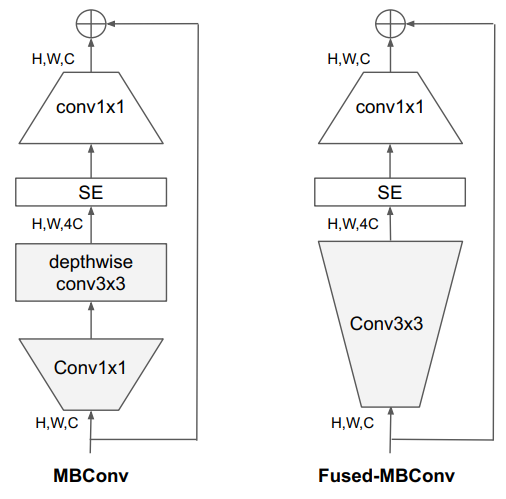
\includegraphics[width=0.5\linewidth]{figures/chapters-imgs/30/fused-mbconv.png}
    \caption{Diagram illustrating the architecture of MBConv and Fused-MBConv, as presented in~\cite{tan2021efficientnetv2}.}
    \label{fig:fused-mbconv}
\end{figure}

In this study, we will utilize the \textit{EfficientNetV2-M} backbone, which comprises roughly $54M$ parameters. This model underwent training for a classification task using the \textit{ImageNet-1K} dataset~\cite{5206848} over 350 epochs. Subsequently, it was retrained on the \textit{ImageNet-21K} dataset~\cite{5206848} for an additional 350 epochs.

\section{Necks}
As illustrated in Figure \ref{fig:net-backbone-neck-head}, the \textit{neck} model plays a crucial role in aggregating features derived from the \textit{backbone}. Its primary function is to gather feature maps from different stages of the backbone, facilitating interaction between high-level and low-level features.
For this work, we will explore two types of \textit{neck} models: the state-of-the-art \textit{BiFPN}~\cite{DBLP:journals/corr/abs-1911-09070} and a variant we introduce, the \textit{CA-BiFPN}, which will be detailed in the Chapter \ref{chap:40}. Before delving into the \textit{BiFPN}~\cite{DBLP:journals/corr/abs-1911-09070} model, it's essential to understand the pioneering neck models that laid the foundation for the \textit{BiFPN} architecture: namely, the \textit{FPN}~\cite{Lin_2017_CVPR}, \textit{PANet}~\cite{DBLP:journals/corr/abs-1803-01534}, and \textit{NAS-FPN}~\cite{DBLP:journals/corr/abs-1904-07392}.

\subsection{FPN}
The prior use of featurized image pyramids~\cite{adelson1984pmi} in object detection was aimed at leveraging their scale-invariance. This unique property allows a model to detect objects over a vast scale range by examining in the pyramid levels. As a result, the detector can generate a multi-scale feature representation where every level, possesses robust semantic value. However, employing this multi-scale feature without an appropriate method of feature fusion can lead to significant semantic discrepancies due to varied depths.
To address this challenge, \textit{Tsung-Yi Lin et al.} introduced~\cite{Lin_2017_CVPR} an architecture that adeptly merges low-resolution features rich in semantics with high-resolution features that are semantically weaker. This is achieved through a top-down pathway combined with lateral connections.\\

\begin{figure}[htb]
    \centering
    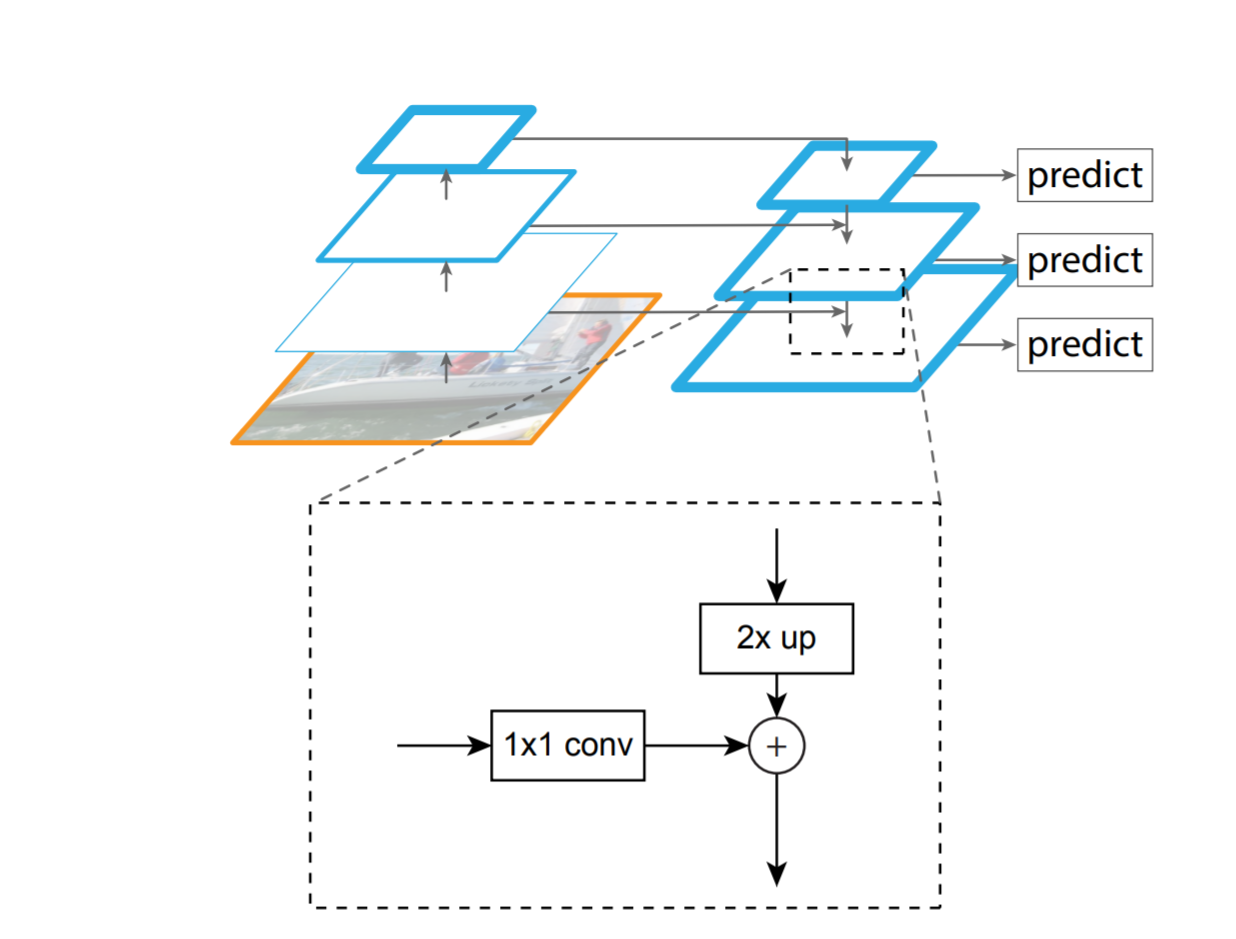
\includegraphics[width=0.65\linewidth]{figures/chapters-imgs/30/fpn-arq.png}
    \caption{Diagram illustrating the architecture FPN, as presented in~\cite{Lin_2017_CVPR}.}
    \label{fig:fpn-arq}
\end{figure}

The architecture proposed, named \textit{FPN} by its creators, incorporates two primary strategies: the Bottom-up pathway and the Top-down pathway with lateral connections. 
In the Bottom-up pathway, the network leverages feature maps extracted from various stages of the backbone. For each of these stages, the network designates a distinct pyramid level. This means that as one progresses through the stages of the backbone, different pyramid levels are determined, capturing features at various resolutions and scales.
Conversely, in the Top-down pathway, each pyramid level undergoes upsampling with a spatial resolution factor of 2. This upsampling is then integrated with the lateral connections originating from the Bottom-up pathway. These lateral connections play a pivotal role in bridging the semantic gap between the features. Specifically, each lateral connection seamlessly combines feature maps, all of the same spatial dimensions, from both the Bottom-up and Top-down pathways. This combination is achieved through element-wise addition. A visual representation of this intricate process can be observed in Figure \ref{fig:fpn-arq}.\\

By intricately merging the Bottom-up and Top-down pathways through the use of lateral connections, the \textit{FPN} architecture achieves a seamless integration of feature maps. These maps, which come from diverse scales and possess varying semantic strengths, are blended harmoniously. This unique integration technique provides the \textit{FPN} with the capability for robust multi-scale object detection. After this fusion process, the various pyramid levels are then channeled into the head detector. Regardless of their original dimensions or scales, these feature maps are standardized to a fixed feature dimension in the final layer.

\subsection{PANet}
Building upon the architecture of the Feature Pyramid Network (FPN)~\cite{Lin_2017_CVPR}, \textit{Shu Liu et al.} extended their research \cite{DBLP:journals/corr/abs-1803-01534} to introduce a more sophisticated architecture termed the \textit{Path Aggregation Network (PANet)}. They pinpointed a significant challenge in the foundational FPN design: a lengthened pathway from the basic structural elements to the most advanced features. This elongated route hinders the extraction of detailed localization information. Notably, accessing features at the foundational levels, which are crucial for pinpointing larger instances, becomes increasingly difficult.\\

In tackling the challenge, the \textit{Bottom-up Path Augmentation} method is adopted. This method amplifies the entire feature hierarchy's localization ability by highlighting the dominant responses of foundational patterns, as show in Figure \ref{fig:panet-arq}. 
Within the \textit{FPN}, feature maps \(P_{i}\) with consistent spatial sizes are utilized. The \textit{PANet} structure then designs a segment. This segment integrates a detailed feature map \(N_{i}\) with a comparatively coarser map \(P_{i+1}\) using lateral pathways, resulting in the updated feature map \(N_{i+1}\). Each of these maps first passes through a convolution with a kernel $3\times 3$ and a stride of 2, leading to a decrease in its spatial dimensionality. After this stage, elements of the feature map \(P_{i+1}\) are fused with the reduced map using lateral pathways. This integrated feature representation is then processed through an additional convolution with a kernel $3\times 3$, giving rise to \(N_{i+1}\) for the following sub-network layers, as illustrated in Figure \ref{fig:panet-block}.

\begin{figure}[htb]
    \centering % <-- added
\begin{subfigure}{0.62\textwidth}
  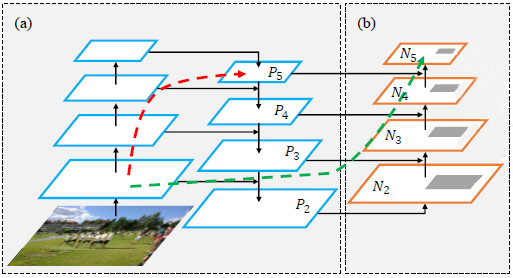
\includegraphics[width=\linewidth]{figures/chapters-imgs/30/panet-arq.jpg}
  \caption{\protect\raggedright Illustration of the PANet Architecture: (a.a) The foundational FPN backbone; (a.b) The Bottom-up path augmentation.}
  \label{fig:panet-arq}
\end{subfigure} % <-- added
\medskip
\begin{subfigure}{0.32\textwidth}
  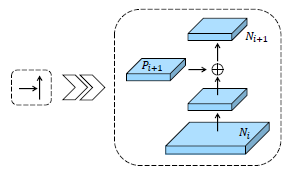
\includegraphics[width=\linewidth]{figures/chapters-imgs/30/panet-block.png}
  \caption{\protect\raggedright Diagram illustrating the PANet architecture for bottom-up path augmentation block.}
  \label{fig:panet-block}
\end{subfigure}
\caption{Diagram illustrating the PANet architecture and its associated proposed fusion feature block, as detailed in~\cite{DBLP:journals/corr/abs-1803-01534}.}
% \label{fig:}
\end{figure}

\subsection{NAS-FPN}
In the study presented by \textit{Golnaz Ghiasi et al.}, they introduced a novel architecture termed \textit{NAS-FPN}~\cite{DBLP:journals/corr/abs-1904-07392}. This architecture leverages an extensive search space to discern the optimal arrangement of unit merge routes. The technique they adopted is based on the Neural Architecture Search (NAS) methodology~\cite{DBLP:journals/corr/ZophL16}, which was previously proposed by \textit{Zoph et al.}~\cite{DBLP:journals/corr/ZophVSL17}. A distinctive feature of this algorithm is its capability to craft modular architectures. Such modular structures can be efficiently replicated and stacked, culminating in a scalable design. Inspired by this modular concept, \textit{Golnaz Ghiasi et al.} designed a search space adept at churning out scalable architectures, especially those generating pyramidal representations.\\

The primary objective of the algorithm under discussion is to identify an enhanced FPN (Feature Pyramid Network) architecture suitable for a specific backbone. This relationship is clearly depicted in Figure \ref{fig:nas-fpn-space}.
\begin{figure}[htb]
    \centering
    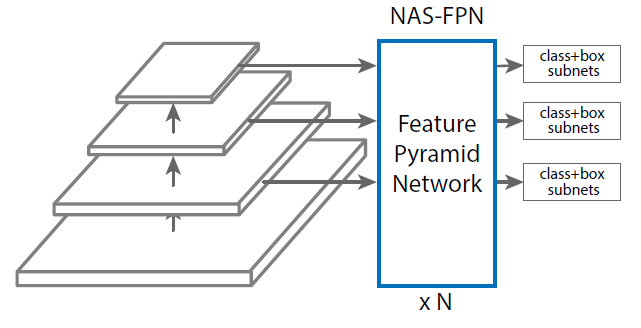
\includegraphics[width=0.4\linewidth]{figures/chapters-imgs/30/nas-fpn-space.png}
    \caption[Diagram illustrating the interconnection between backbone stages and the NAS-FPN search spaces.]{Diagram illustrating the interconnection between backbone stages and the NAS-FPN search spaces. The modular nature of the NAS-FPN architecture allows it to be stacked $N$ times, potentially improving its accuracy. A comprehensive description of this stacking mechanism can be found in~\cite{DBLP:journals/corr/abs-1904-07392}.}
    \label{fig:nas-fpn-space}
\end{figure}
In the realm of FPN, a designated search space is formulated to generate feature pyramid representations. Within this framework, Neural Architecture Search (NAS) deploys a controller. This controller, utilizing reinforcement learning, is tasked with selecting the most optimal model architectures from the defined search space. A significant characteristic of the identified FPN model is its inherent scalability. To achieve larger, integrated architectures, the model can replicate itself $N$ times, subsequently merging these instances into a unified, comprehensive structure.\\

In the NAS-FPN search space, the last layer of each group of feature layers from the backbone serves as the input to the initial pyramid network. Subsequently, the outputs from this first pyramid network become the inputs for the succeeding pyramid network. When considering the input feature within the search space, it is routed through a pyramid network composed of a sequence of merging cells. These cells facilitate cross-scale connections, as depicted in Figure \ref{fig:nas-merge-cell}. The final outputs are then expanded into multiscale feature representations. Notably, this architectural design allows for iterative stacking, which can potentially enhance accuracy.

\begin{figure}[htb]
    \centering
    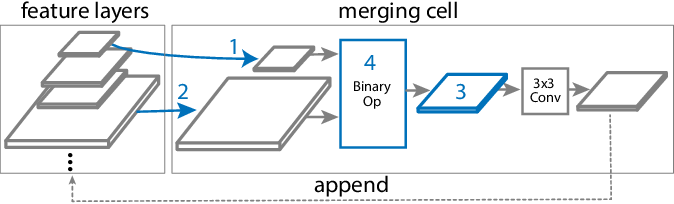
\includegraphics[width=0.6\linewidth]{figures/chapters-imgs/30/nas-merge-cell.png}
    \caption{Diagram showcasing the merging cell utilized within the search space, further elaborated in~\cite{DBLP:journals/corr/abs-1904-07392}.}
    \label{fig:nas-merge-cell}
\end{figure}

The process employed by the merging cell within the search spaces can be delineated into four pivotal steps:
\begin{enumerate}[label=(\Roman*)]
    \item Select a feature layer \( h_i \) from the available candidates.
    \item Choose another feature layer \( h_j \) from the candidates, ensuring no repetition.
    \item Determine the desired output feature resolution.
    \item Opt for a binary operation, either summation or global pooling, to amalgamate \( h_i \) and \( h_j \) chosen in steps (I) and (II). This amalgamation produces a feature layer resonating with the resolution specified in step (III).
\end{enumerate}
All these steps are illustratively represented in Figure \ref{fig:nas-merge-cell}.\\

Figure \ref{fig:nas-search-space} presents the finalized search spaces. Notably, the architecture with the highest performance is represented by the last graph (f) within the figure.
\begin{figure}[htb]
    \centering
    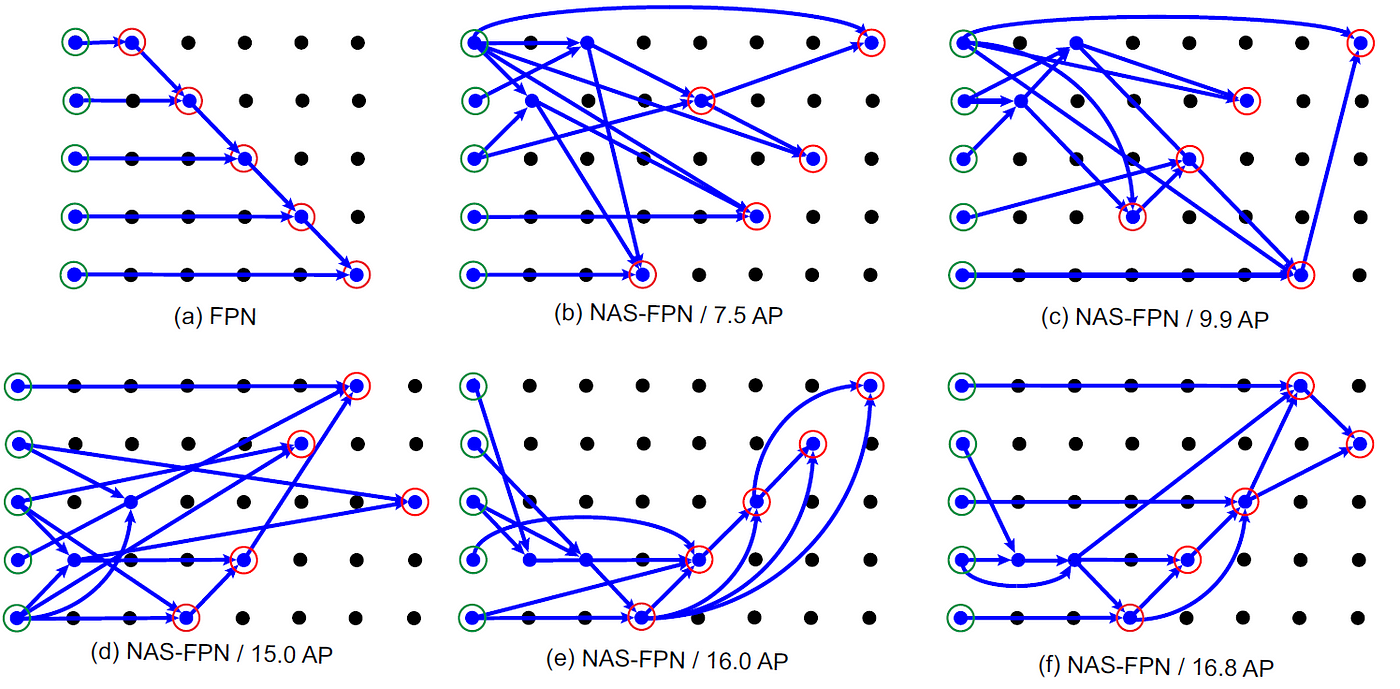
\includegraphics[width=0.9\linewidth]{figures/chapters-imgs/30/nas-search-space.png}
    \caption[The diagram depicts various architecture graphs of NAS-FPN within the search space.]{\protect\raggedright The diagram depicts various architecture graphs of NAS-FPN within the search space. Each dot symbolizes a feature layer, with feature layers in the same row sharing a uniform resolution. Arrows delineate connections between internal layers. The initial graph (a) corresponds to the baseline FPN architecture, while graphs (b-f) represent the 7-cell NAS-FPN architectures identified by the NAS controller. Image and caption sourced from~\cite{DBLP:journals/corr/abs-1904-07392}.}
    \label{fig:nas-search-space}
\end{figure}

\subsection{BiFPN}
The imperative nature of devising an architectural framework that offers scalability in detection, while simultaneously ensuring enhanced accuracy and superior efficiency across an expansive range of resource constraints, has driven researchers to seek innovative solutions. In light of this, \textit{Mingxing Tan et al.} introduced the model termed \textit{Bi-Directional Feature Pyramid Network (BiFPN)}~\cite{DBLP:journals/corr/abs-1911-09070}. This model endeavors to achieve elevated performance metrics in one-stage detectors. It does so by harnessing the capabilities of an efficient multi-scale feature fusion coupled with learnable weights. These weights are strategically employed to discern and adapt to the significance of varied input features.\\

In this study, the researcher critically evaluated the \textit{Multi-Scale Feature Representations} as proposed by the NAS-FPN model~\cite{DBLP:journals/corr/abs-1904-07392}. It was observed that the execution of this model necessitates a disproportionately high consumption of resources, primarily due to the vastness of its search space. Furthermore, when inspecting architectures such as FPN~\cite{Lin_2017_CVPR} and NAS-FPN~\cite{DBLP:journals/corr/abs-1904-07392}, there seems to be a discrepancy in the manner in which different input features are fused, resulting in an inconsistent output feature fusion.
To address these shortcomings and augment the model's efficiency, the BiFPN was introduced, which incorporates \textit{cross-scale connections}. These connections are specifically designed to rectify the aforementioned inefficiencies in the previously discussed architectures. The optimizations encapsulated within BiFPN include:
\begin{enumerate}
    \item The elimination of nodes possessing only a singular input edge. This is orchestrated with the objective of eschewing nodes that do not actively participate in the fusion of different feature maps, thus ensuring that only the significant nodes with multiple connections contribute to feature amalgamation.
    
    \item The integration of an additional edge that extends from the original input feature maps to the corresponding output node, provided they reside on the same hierarchical level. This is pursued to facilitate a more comprehensive feature fusion without necessitating the introduction of a plethora of operators.
    
    \item The incorporation of a bi-directional pathway (both top-down and bottom-up) within a singular feature network layer. This layer is then replicated numerous times to foster an enriched high-level feature fusion process.
\end{enumerate}
A graphic representation detailing these optimizations, showcasing BiFPN as the feature network, can be found in Figure \ref{fig:bifpn-net}.

\begin{figure}[htb]
    \centering
    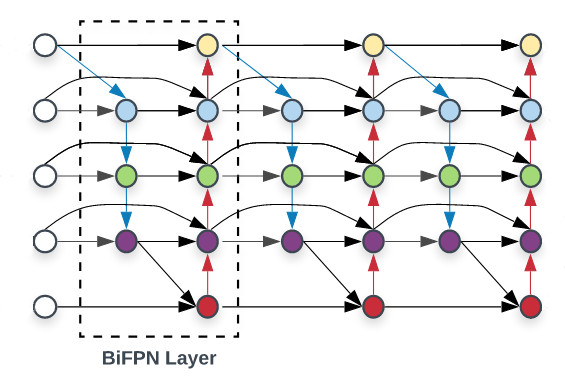
\includegraphics[width=0.7\linewidth]{figures/chapters-imgs/30/bifpn-net.jpg}
    \caption{\protect\raggedright Diagram illustrating of BiFPN as the feature network. Image adapted from~\cite{wang2023internimage}.}
    \label{fig:bifpn-net}
\end{figure}

In the preceding architectures, there is a discernible uniformity in the treatment of input features. This homogeneity often overlooks the nuanced significance that some features might possess over others. Contrary to this general approach, BiFPN employs a strategy that allocates a unique weight to each input. This allocation is not arbitrary; rather, it is meticulously designed to facilitate the network's learning of the relative importance of each input feature. This weighting mechanism is encapsulated in the methodology termed \textit{Fast Normalized Fusion}, which is described as:
\begin{equation}
O=\sum_i \frac{w_i}{\epsilon+\sum_j w_j} \cdot I_i,
\end{equation}
In the above equation, \(I_i\) delineates the \(i\)-th fused feature map. The term \(w_i\) represents the weight of the corresponding feature map, and to ensure its non-negativity, a Rectified Linear Unit (ReLU) is applied post determination of each \(w_i\). The constant \(\epsilon=0.0001\) is judiciously incorporated to circumvent potential numerical instabilities that might arise during calculations.

\section{Object Instance Segmentation}
Segmenting and identifying distinct objects within images is a foundational pillar of computer vision. This process, often termed as Object Instance Segmentation, is instrumental in equipping machines with the capability to delineate and recognize individual entities, as explained in the last chapter. This section traces this evolutionary path, elucidating the mechanisms and novelties of R-CNN and its descendants: Fast R-CNN, Faster R-CNN, and Mask R-CNN. Each algorithm brought forth incremental refinements, ensuring faster processing times, enhanced accuracy, and the ability to tackle more nuanced tasks like instance segmentation.

\subsection{R-CNN}
In the realm of object detection, the R-CNN (Regions with Convolutional Neural Networks) methodology stands as a pioneering contribution. It was introduced by \textit{Ross Girshick et al.} in their work \cite{DBLP:journals/corr/GirshickDDM13}, and it skillfully integrates region proposals with the functionalities of convolutional neural networks. The architecture's essence is captured within three primary modules:
\begin{enumerate}
    \item \textit{Region Proposal}: This module allow to generate around 2000 category-independent region proposals for each image. This  is achieved using the \textit{Selective Search}~\cite{Uijlings2013} algorithm, which is based on a bottom-up segmentation approach.
    \item \textit{Feature Extraction}: Each of these region proposals is then warped to a fixed size and passed through a pre-trained CNN to extract a 4096-dimensional feature vector.
    \item \textit{Classification}: A set of class-specific linear Support Vector Machines~(SVMs) is trained using the above feature vectors. For each region, the SVM outputs a classification score, and bounding box regressors are used to fine-tune the object's location.
\end{enumerate}

A visual representation encapsulating these modules is presented in Figure \ref{fig:rcnn}.

\begin{figure}[htb]
    \centering
    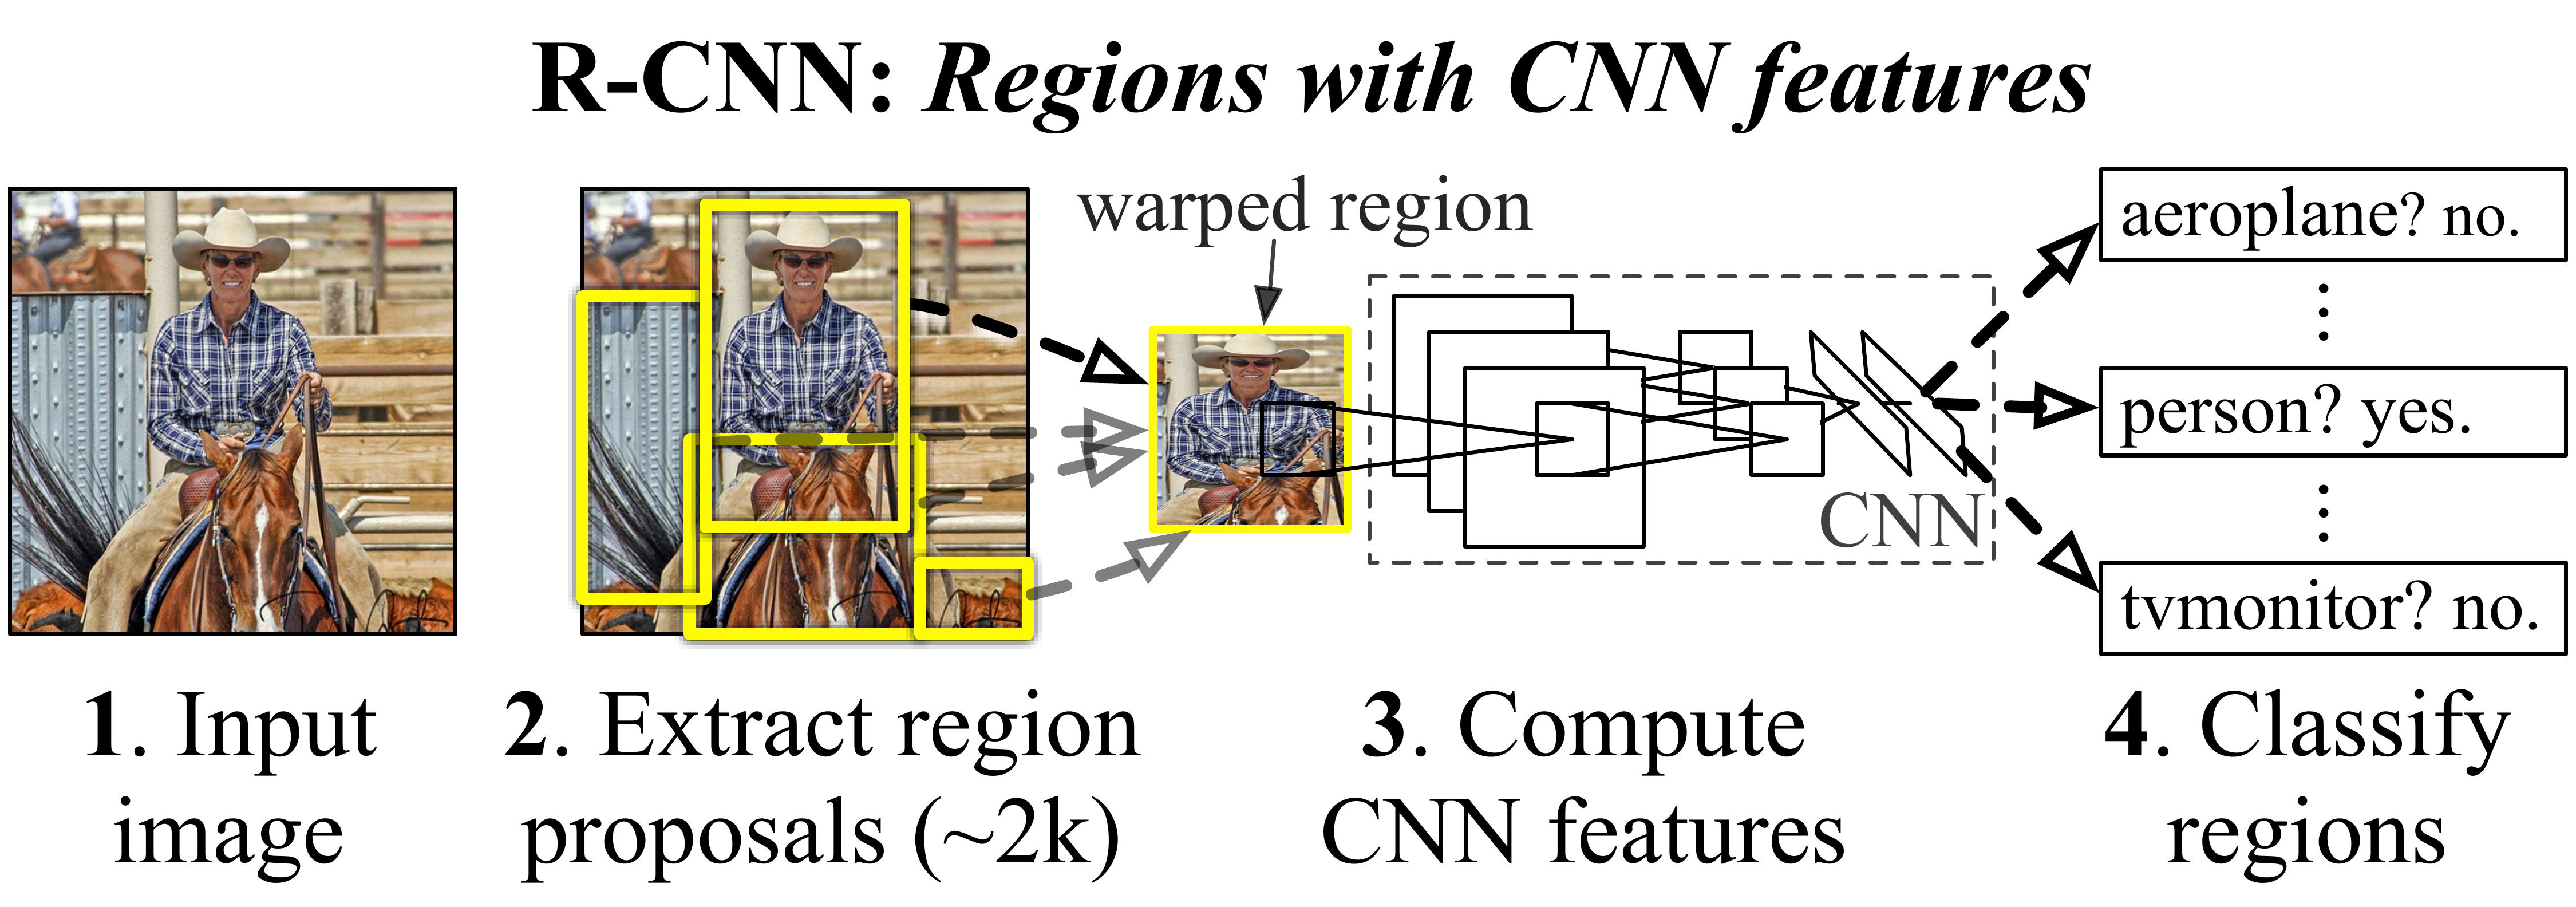
\includegraphics[width=0.7\linewidth]{figures/chapters-imgs/30/rcnn.png}
    \caption{The object detection framework as delineated by R-CNN. Image adapted from~\cite{DBLP:journals/corr/GirshickDDM13}.}
    \label{fig:rcnn}
\end{figure}

\subsection{Fast R-CNN}
Despite the groundbreaking innovations introduced by the architecture of R-CNN~\cite{DBLP:journals/corr/GirshickDDM13}, it exhibits several notable limitations. Chief among these are its space and time-intensive multi-stage pipeline training, the prolonged detection times during the inference phase, and the absence of shared computation in the forward pass for each object proposal. Recognizing these challenges, Ross Girshick introduced the Fast R-CNN architecture~\cite{DBLP:journals/corr/Girshick15}, which employs a single-stage training algorithm. This new algorithm concurrently learns to classify object proposals and finetune their spatial positions.\\

In the operational flow of the Fast R-CNN architecture, the input image initially undergoes processing through multiple convolutional and max pooling layers, leading to the generation of a feature map. Subsequently, for each object proposal, the architecture incorporates a Region Of Interest (RoI) pooling layer, which is pivotal in extracting a fixed-length feature vector from the aforesaid feature map. This feature vector is then forwarded to a series of fully connected layers, culminating in two distinct output layers. The first output layer is tasked with generating softmax probability estimates over $K$ object classes, plus a separate class for the background. The second layer, conversely, outputs four real-valued coordinates for each of the $K$ object classes. These coordinates effectively refine the bounding-box positions corresponding to each class. A schematic representation of this intricate process is delineated in Figure \ref{fig:fast-rcnn}.

\begin{figure}[htb]
    \centering
    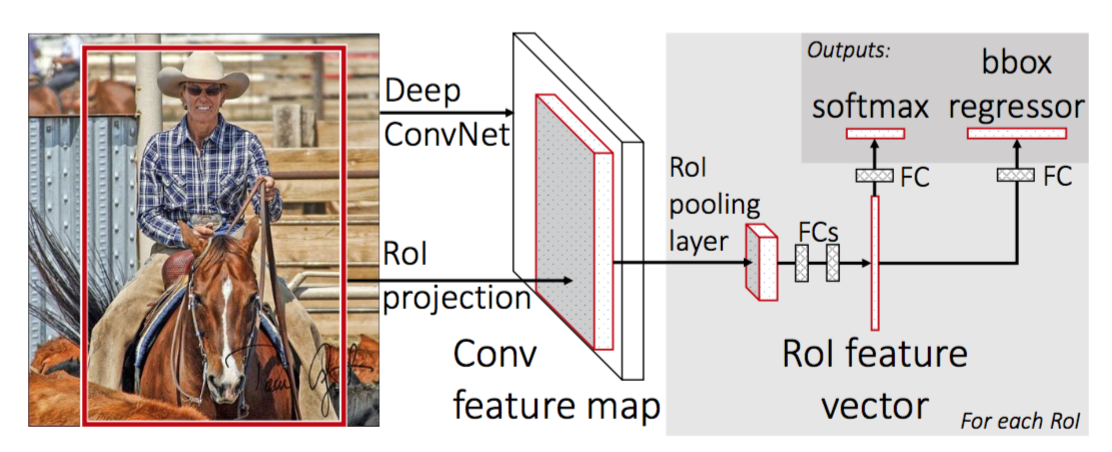
\includegraphics[width=0.7\linewidth]{figures/chapters-imgs/30/fast-rcnn.png}
    \caption{An overview of the Fast R-CNN architecture, as sourced from~\cite{DBLP:journals/corr/Girshick15}.}
    \label{fig:fast-rcnn}
\end{figure}

Within the scope of the described processes, the introduction of the \textit{Region of Interest (RoI) pooling layer} emerges as a crucial innovation. This RoI pooling layer employs the max pooling operator to transform features encapsulated within any valid region of interest into a compact feature map of a consistent spatial dimension, represented as \(H \times W\). Notably, the dimensions \(H\) and \(W\) function as layer hyperparameters and maintain independence from any specific RoI. Every individual RoI is characterized by a quadruple \((r, c, h, w)\), which demarcates its top-left corner with coordinates \((r, c)\) and further defines its dimensions with height \(h\) and width \(w\). Here, the operational principle of the max pooling technique entails partitioning the \(h \times w\) RoI window into an \(H \times W\) sub-window grid. Each of these sub-windows approximates a size of \(h/H \times w/W\), and the values within them are subsequently max-pooled into the corresponding grid cell of the output feature map.\\

The epithet \textit{fast} in the architecture alludes to its refinement optimized for detection. The underlying objective is the holistic training of all weights during the back-propagation phase. Fast R-CNN achieves this by harnessing a single-stage training process in tandem with a multi-task loss. This multi-task loss is intrinsically tied to the aforementioned dual output layers. For the primary output layer, a discrete probability distribution, symbolized as \(p = (p_0, ..., p_K)\), is formulated for each RoI. This distribution is derived from the softmax function applied over the \(K+1\) outputs emanating from a fully connected layer. Pertaining to the secondary output layer, bounding-box regression offsets are parameterized as \(t^k=\left(t_{\mathrm{x}}^k, t_{\mathrm{y}}^k, t_{\mathrm{w}}^k, t_{\mathrm{h}}^k\right)\) for the \(k\)-th object class. Then, given a labeled RoI associated with a ground-truth class \(u\) and a corresponding bounding-box regression target \(v\), the encompassing multi-task loss \(L\) for both classification and bounding-box regression can be expressed as:
\begin{equation}
L\left(p, u, t^u, v\right)=L_{\mathrm{cls}}(p, u)+\lambda[u \geq 1] L_{\mathrm{reg}}\left(t^u, v\right) \label{eq:fast-rcnn}.
\end{equation}
In this equation, \(\lambda\) functions as a hyperparameter modulating the equilibrium between the dual task losses. The Iverson bracket indicator function, denoted by \([u \geq 1]\), evaluates to 1 when the condition \(u \geq 1\) is met and 0 otherwise. Further, \(L_{\mathrm{cls}}(p, u)=-\log p_u\) signifies the log loss for the genuine class \(u\). The bounding-box regression loss, \(L_{\mathrm{reg}}\), is ascribed to the target \(u, v =\left(v_{\mathrm{x}}, v_{\mathrm{y}}, v_{\mathrm{w}}, v_{\mathrm{h}}\right)\) and its predicted counterpart \(t^u=\left(t_{\mathrm{x}}^u, t_{\mathrm{y}}^u, t_{\mathrm{w}}^u, t_{\mathrm{h}}^u\right)\), and is given by:
\begin{equation}
L_{\mathrm{reg}}\left(t^u, v\right)=\sum_{i \in\{\mathrm{x}, \mathrm{y}, \mathrm{w}, \mathrm{h}\}} \operatorname{smooth}_{L_1}\left(t_i^u-v_i\right)
\end{equation}
The function \(\operatorname{smooth}_{L_1}(x)\) is defined as:
\begin{equation}
\operatorname{smooth}_{L_1}(x)= \begin{cases}0.5 x^2 & \text { if }|x|<1 \\ |x|-0.5 & \text { otherwise }\end{cases}.
\end{equation}

\subsection{Faster R-CNN}
Leveraging the innate potential of Fast R-CNN for generating region proposals, \textit{Shaoqing Ren et al.} formulated an integrated architecture, termed as Faster R-CNN~\cite{DBLP:journals/corr/RenHG015}. This architecture comprises two pivotal modules: (I) Region Proposal Networks (RPNs) and (II) the Fast R-CNN detector, as depicted in Figure \ref{fig:faster-rcnn}. The overarching objective of these networks is to engender region proposals potentially encapsulating objects.

\begin{figure}[htb]
    \centering
    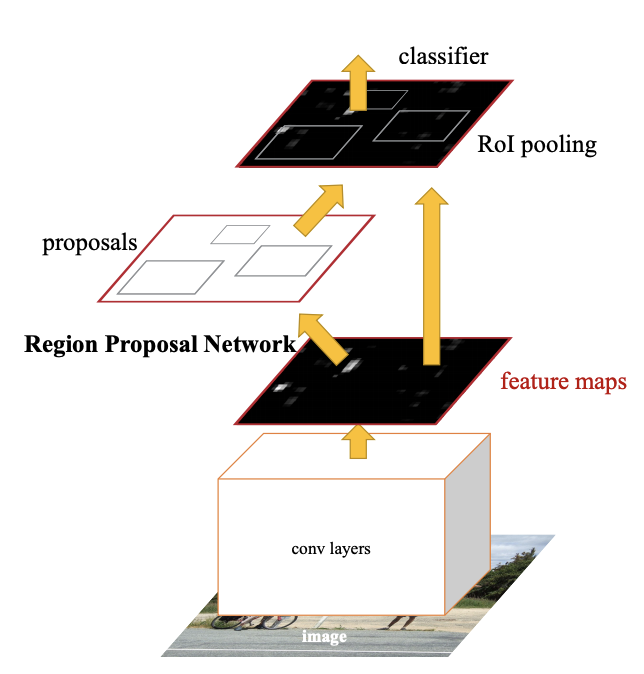
\includegraphics[width=0.5\linewidth]{figures/chapters-imgs/30/faster-rcnn.png}
    \caption[Faster R-CNN represents a unified network dedicated to object detection.]{Faster R-CNN represents a unified network dedicated to object detection, wherein the RPN module acts as the network's \textit{attention}. Image and caption have been sourced from~\cite{DBLP:journals/corr/RenHG015}.}
    \label{fig:faster-rcnn}
\end{figure}

Delving deeper, the Region Proposal Networks are designed to intake an image of arbitrary dimensions and subsequently output an array of rectangular object proposals, each quantified with an objectness score. To achieve this, the RPN processes a diminutive network atop the convolutional feature map that emerges from the terminal shared convolutional layer. This concise network imbibes an $n \times n$ spatial window from the originating convolutional feature map. Every sliding window is then transposed into a lower-dimensional feature, subsequently funneled into two sibling fully-connected layers. These layers are tailored for box-regression and box-classification, respectively. For each sliding window locale, simultaneous predictions are made for multiple region proposals, with the upper bound of possible proposals for any given location symbolized by $k$. These $k$ proposals are parameterized in correlation to $k$ reference boxes, denominated as \textit{anchors}. Notably, every anchor is centralized at the respective sliding window, possessing a defined scale and aspect ratio, as illustrated in Figure \ref{fig:faster-rcnn-anchors}.

\begin{figure}[htb]
    \centering
    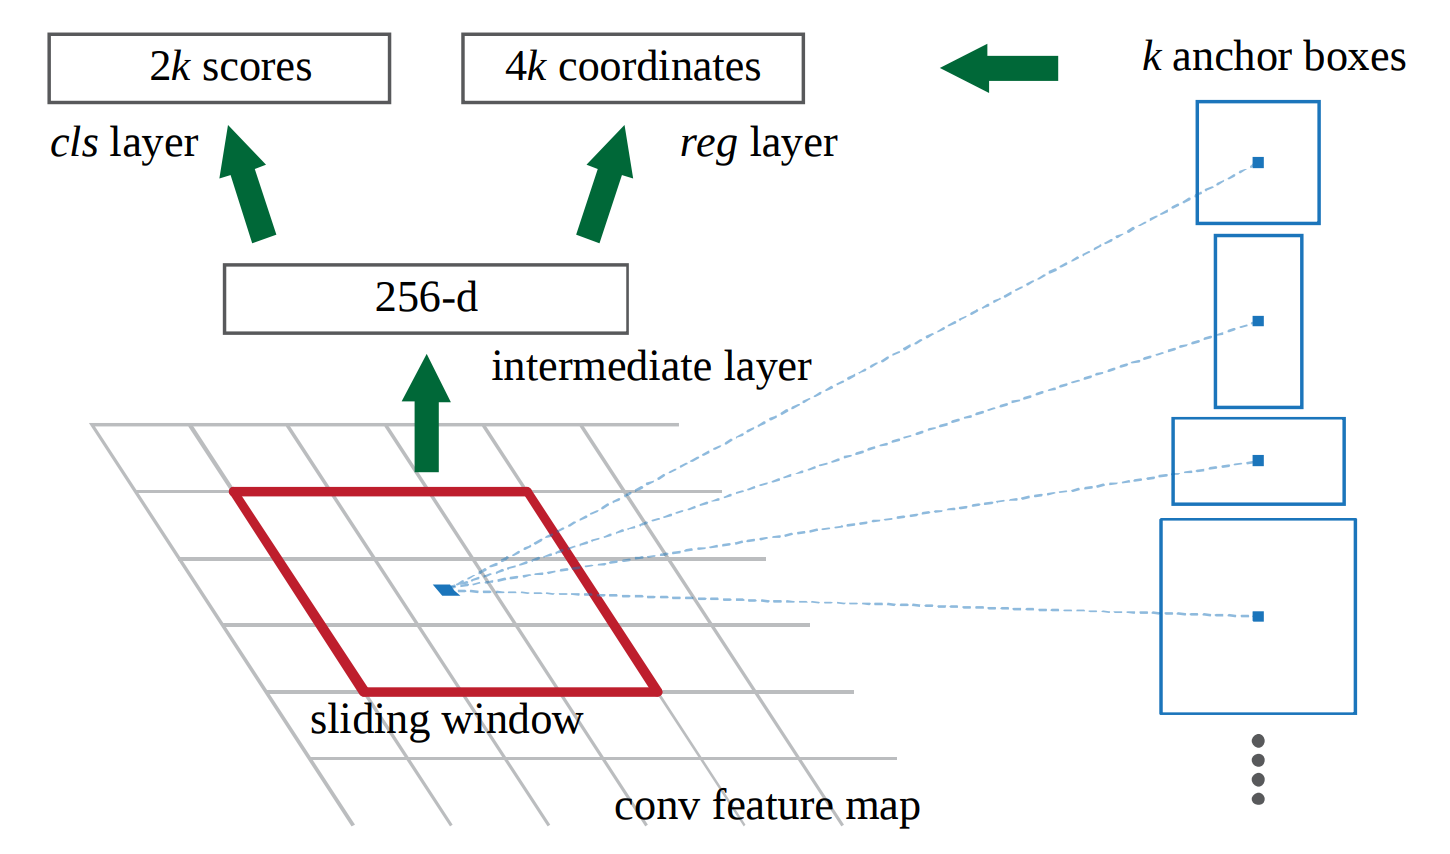
\includegraphics[width=0.7\linewidth]{figures/chapters-imgs/30/faster-rcnn-anchors.png}
    \caption{The architecture of the Region Proposal Network (RPN). Image and caption sourced from~\cite{DBLP:journals/corr/RenHG015}.}
    \label{fig:faster-rcnn-anchors}
\end{figure}

In a quest to uphold the \textit{fast} essence intrinsic to the Fast R-CNN~\cite{DBLP:journals/corr/Girshick15}, the Faster R-CNN architecture embodies a revamped multi-task loss function for the Region Proposal Network. This is achieved by introducing a binary class assignment for every anchor, distinguishing it as either an object or a non-object. The resultant loss to be minimized can be represented as:
\begin{equation}
L\left(\left\{p_i\right\},\left\{t_i\right\}\right)=\frac{1}{N_\mathrm{cls}} \sum_i L_\mathrm{cls}\left(p_i, p_i^*\right) +\lambda \frac{1}{N_{\mathrm {reg}}} \sum_i p_i^* L_{\mathrm{reg}}\left(t_i, t_i^*\right) \label{eq:faster-rcnn}
\end{equation}
Here, $i$ signifies the anchor's index within a mini-batch and $p_i$ denotes the predicted likelihood of anchor $i$ being classified as an object. The ground-truth label, $p_i^*$, is set to 1 if the anchor is identified as positive, and 0 if negative. Meanwhile, $t_i$ stands for a vector detailing the four parameterized coordinates of the projected bounding box. In contrast, $t_i^*$ designates the ground-truth box linked with a positive anchor. The terms $L_{\mathrm{cls}}$ and $L_{\mathrm{reg}}$ mirror those described in equation (\ref{eq:fast-rcnn}). They are normalized by factors $N_\mathrm{cls}$ (referring to the mini-batch size) and $N_\mathrm{reg}$ (pertaining to the total anchor locations). Lastly, \(\lambda\) operates as a hyperparameter orchestrating the balance between the twin task losses.

\subsection{Mask R-CNN}
In their research, \textit{Kaiming He et al.} sought to adapt the architecture of the Faster R-CNN to cater to instance segmentation tasks. The method they introduced, named Mask R-CNN~\cite{DBLP:journals/corr/HeGDG17}, integrates an additional branch designed specifically to predict segmentation masks for each Region of Interest (RoI). This branch operates concurrently with the existing branches focused on classification and bounding box regression, as depicted in Figure \ref{fig:mask-rcnn-arq}.\\

\begin{figure}[htb]
    \centering
    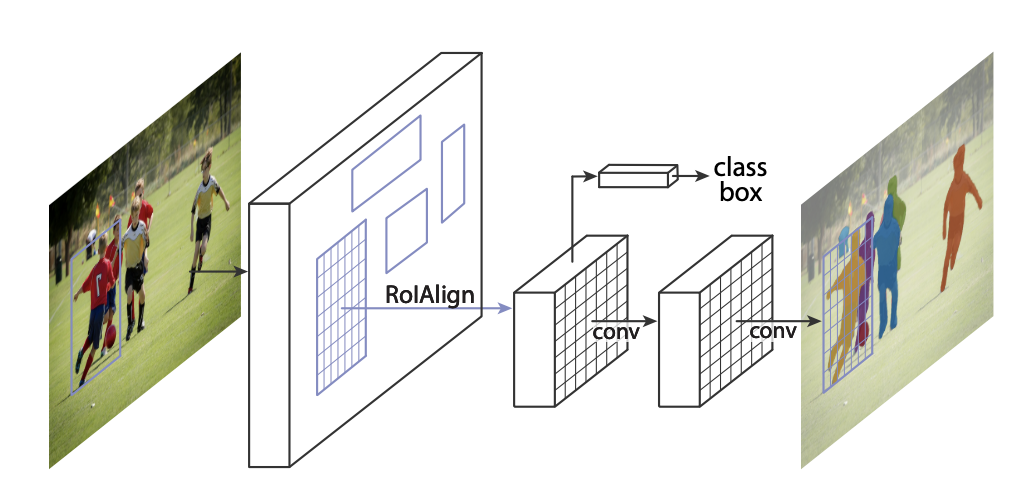
\includegraphics[width=0.7\linewidth]{figures/chapters-imgs/30/mask-rcnn-arq.png}
    \caption{The architecture of Mask R-CNN, as sourced from \textit{Kaiming He et al.}~\cite{DBLP:journals/corr/HeGDG17}.}
    \label{fig:mask-rcnn-arq}
\end{figure}

The architecture of Mask R-CNN builds upon the foundational structure of Faster R-CNN. While the Faster R-CNN is responsible for the class label and bounding-box prediction, the Mask R-CNN integrates a novel branch dedicated to outputting the object mask. This mask is distinct from the class and bounding box outputs, necessitating a more intricate spatial layout extraction of an object. The branch is designed to encode \(K\) binary masks, each of resolution \(m \times m\), one corresponding to each of the \(K\) classes. The intricate spatial structure of the masks is addressed by the inherent pixel-to-pixel correspondence that convolutions offer. Within this architecture, an \(m \times m\) mask is predicted for each RoI using a Fully Convolutional Network (FCN). This approach ensures that each layer in the mask branch retains the explicit \(m \times m\) object spatial layout, avoiding its reduction into a vector representation devoid of spatial dimensions.
One significant innovation in the Mask R-CNN is its acknowledgment of the pixel-to-pixel alignment between network inputs and outputs, an aspect overlooked by the RoIPool utilized in the Fast R-CNN architecture. To address this, Mask R-CNN incorporates a novel RoI layer, termed RoIAlign. RoIAlign serves to rectify the severe quantization inherent in RoIPool, ensuring a precise alignment of the extracted features with the input. The principal objective of this layer is to eschew any quantization of the RoI boundaries or bins. Instead, it employs bilinear interpolation to accurately compute the values of the input features at four systematically sampled locations within each RoI bin, as depicted in Figure \ref{fig:mask-rcnn-roi}.\\

\begin{figure}[htb]
    \centering
    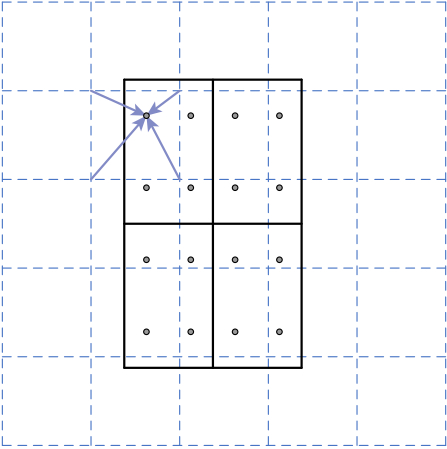
\includegraphics[width=0.3\linewidth]{figures/chapters-imgs/30/mask-rcnn-roi.jpg}
    \caption[RoIAlign design.]{\protect\raggedright RoIAlign: The dashed grid symbolizes a feature map, with the solid lines representing an RoI (comprising 2×2 bins in this instance), and the dots marking the four sampling points in each bin. RoIAlign determines the value of each sampling point through bilinear interpolation from the adjacent grid points on the feature map. Crucially, no quantization is applied to any coordinates related to the RoI, its bins, or the sampling points. Image and caption sourced from~\cite{DBLP:journals/corr/HeGDG17}.}
    \label{fig:mask-rcnn-roi}
\end{figure}

The training phase for the Mask R-CNN method introduces a composite multi-task loss for each sampled RoI, formulated as \(L = L_{\mathrm{cls}} + L_{\mathrm{reg}} + L_{\mathrm{mask}}\). Here, \(L_{\mathrm{cls}}\) and \(L_{\mathrm{reg}}\) remain consistent with those detailed in equation (\ref{eq:faster-rcnn}). \(L_{\mathrm{mask}}\) is the average binary cross-entropy loss. Notably, for an RoI correlated with the ground-truth class \(k\), \(L_{\mathrm{mask}}\) is solely defined on the \(k\)-th mask. This unique definition of the loss \(L_{\mathrm{mask}}\) empowers the network to produce masks for each class without any class competition.